\section{Seq2Seq ASR with Attention}

\begin{frame}[allowframebreaks]{Seq2Seq ASR with Attention}

\textbf{Encoder–Decoder Overview:}
\begin{itemize}
    \item \textbf{Encoder:} Processes the input acoustic features (e.g., Mel-spectrograms) and encodes them into a sequence of hidden representations.
    \item \textbf{Decoder:} Generates the output transcription, one token at a time, conditioned on the encoder outputs and previous decoder states.
    \item \textbf{Attention Mechanism:} Allows the decoder to focus on relevant parts of the input sequence at each decoding step, improving alignment and performance.
\end{itemize}

\begin{figure}[h]
    \centering
    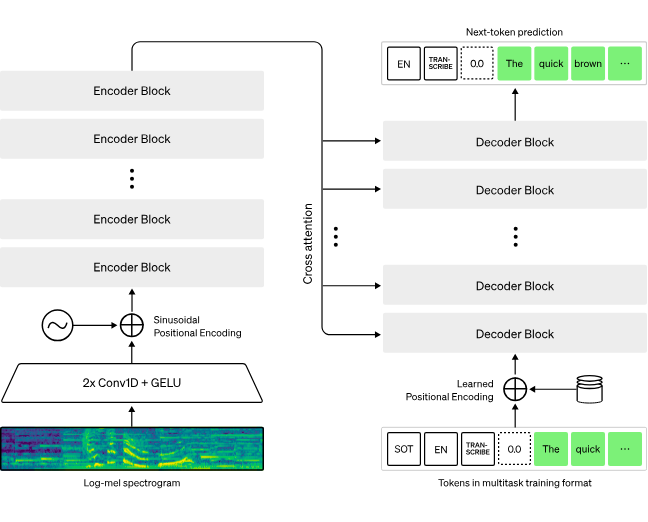
\includegraphics[width=\textwidth,height=0.8\textheight,keepaspectratio]{images/audio-nlp/seq2seq_attention_architecture.png}
    \caption*{Seq2Seq ASR with Attention: Encoder-Decoder Architecture}
\end{figure}

\framebreak

\textbf{Attention Alignment:}

At each decoder time step $t$, the attention mechanism computes a context vector as a weighted sum of encoder outputs. The weights $\alpha_{t,s}$ represent the alignment between decoder step $t$ and encoder position $s$:

\begin{equation}
    \alpha_{t,s} = \frac{\exp(e_{t,s})}{\sum_{s'} \exp(e_{t,s'})}
\end{equation}

where $e_{t,s}$ is the attention score (e.g., computed via a feedforward network) between decoder state at time $t$ and encoder output at position $s$.

\begin{figure}[h]
    \centering
    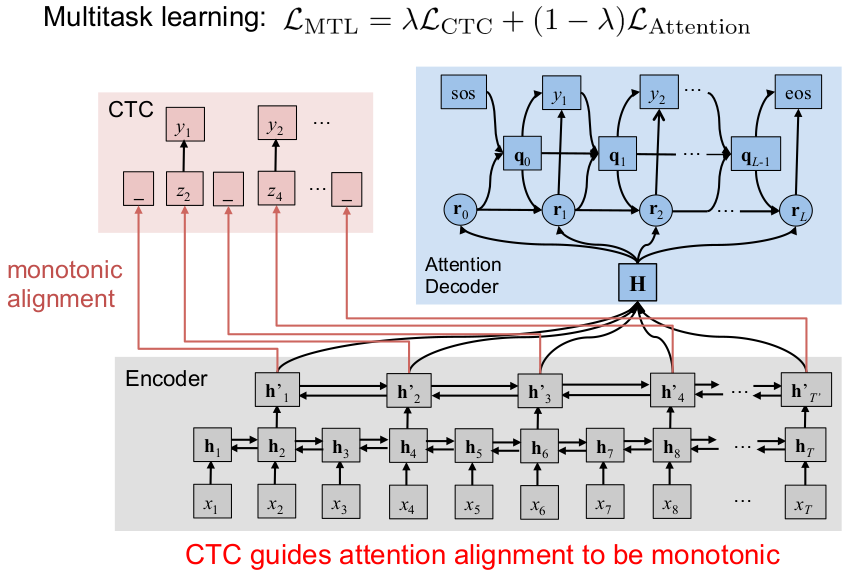
\includegraphics[width=\textwidth,height=0.8\textheight,keepaspectratio]{images/audio-nlp/attention_alignment.png}
    \caption*{Visualization of Attention Alignment}
\end{figure}

\framebreak

\textbf{Example: Listen, Attend and Spell (LAS) on ``hello world''}

\begin{itemize}
    \item The encoder processes the audio features for the phrase ``hello world''.
    \item At each decoding step, the attention mechanism aligns the decoder to the relevant audio frames.
    \item The decoder outputs the transcription character by character (or subword by subword), e.g., ``h'', ``e'', ``l'', ``l'', ``o'', `` '', ``w'', ``o'', ``r'', ``l'', ``d''.
\end{itemize}

% \begin{figure}[h]
%     \centering
%     \includegraphics[width=\textwidth,height=0.8\textheight,keepaspectratio]{images/audio-nlp/las_hello_world_example.png}
%     \caption*{LAS Attention Alignment for ``hello world''}
% \end{figure}

\end{frame}